\section{Multi-segment Ethernet and STP}
\subsection{Multi-segment}

To solve issues with collisions it is neccessary to split the network into different domains each with their own collision domains. This was made possible with the introduction of switches which segmented the network on the Link layer (OSI Level 2) in 1990 by Kalpana, which was later acquired by Cisco. The segmentation resulted in traffic no longer being broadcast across multiple nodes, and at the extreme each node is connected directly to a network switch forming a micro segment. In 1998 full 8 wire twisted pair wires were introduced which allowed for Pysical layer (OSI Level 1) segmentation as the cables were now full duplex. In the years since the price of CAT 5 cables and switches has dropped, and eventually the older technologies were phased out in most networks, removing all potential for collisions. To ensureAs a consequence of the collision free networks it became possible to exceed 10 Mbps and modern networking cards support 100 Mbps at a minimum and 1 Gbps is becoming more common. To insure thees network speeds there was made spanning-tree protocol (STP) which is building for making forwarding topology free-loop and for reducing broadcast radiation. 

\subsection{Spanning-tree protocol}
The idea behind the STP protocol is to have only one way from one node to another one. As in the Figure \ref{fig:STP} A is before the algorithm B is after the algorithm. The STP finds the fastest and loop-free path between two nodes.

Kruskal's algorithm:

\begin{enumerate}
	\item Sort the edges by weight, increasing, and add them to a list.
	\item Add the edge with the lowest weight from the list and remove it from the list hereafter.	
	\item Add the next edge with the lowest weight if adding the edge does not create a circle and remove it from the list hereafter.
	\item Repeat 4 step until a minimum spanning tree has been formed.
\end{enumerate}

The algorithm was made during the course using networkx library in python the Figure\ref{fig:STP} shows graphical example for our implementation of Kruskal's algorithm.

\begin{figure}[H]\label{}
	\centering
	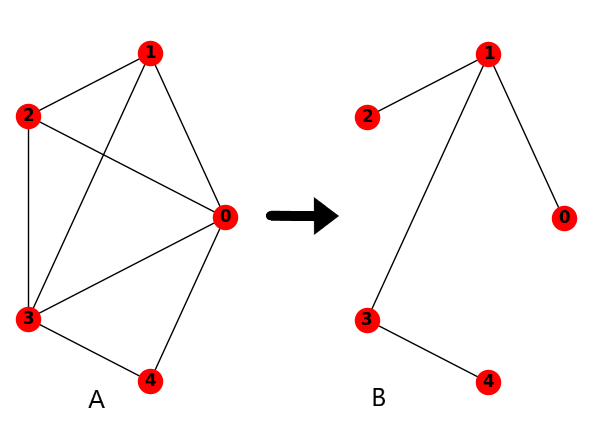
\includegraphics[scale=0.5]{realTimeEthernet/Image/STP.png}
	\caption{Spanning-tree protocol exercise}
	\label{fig:STP}
\end{figure}
